\chapter{Projeto e verificação do sistema de aquisição}\label{cap:sistema}

O sistema usado na coleta em campo tem quatro programas: o \textit{firmware} do transmissor, que mede a vibração na máquina; o do \textit{gateway}, que recebe as medições pelo rádio, as grava e as entrega; a API, que guarda os dados num banco PostgreSQL; e o aplicativo de mesa, pelo qual o operador configura os dispositivos e acompanha as coletas. O transmissor e o \textit{gateway} usam microcontroladores ESP32 e trocam dados por LoRa, na faixa de \SI{433}{\mega\hertz}. Em cada ciclo de medição, o transmissor envia pelo rádio uma telemetria, com os indicadores calculados sobre a janela de sinal e o estado do dispositivo, e o \textit{gateway} e a API gravam cada telemetria recebida como uma leitura. O \textit{gateway} se comunica com a API pela rede Wi-Fi do local, e nenhuma parte do sistema depende de acesso à internet. Depois da primeira gravação dos \textit{firmwares}, os dois dispositivos são configurados sem cabo, pelo aplicativo. O sistema foi desenvolvido neste trabalho a partir de agosto de 2026. A primeira versão do \textit{firmware}, aqui chamada de \textit{firmware} de bancada, enviava pelo rádio apenas os indicadores, e a versão da coleta, descrita nesta seção, envia também a janela de sinal bruto.

A versão usada na coleta foi verificada por testes automatizados no computador e por ensaios de ponta a ponta na bancada, na madrugada e na manhã do dia da coleta. Em 7 de novembro de 2026, passaram os \sisTestesCasos\ casos de teste do \textit{firmware}, dos quais \sisTestesCampoCasos\ se aplicam a funções dos \textit{firmwares} da coleta. Nos ensaios, o banco de teste recebeu \sisBancoLeituras\ leituras, nenhuma duplicada, e \sisBancoJanelasCompletas\ das \sisBancoJanelas\ janelas chegaram com todos os fragmentos. As leituras recebidas durante uma queda da API de \sisQuedaApiS~s foram entregues depois que ela voltou (seção~\ref{sec:sis-verificacao}).

\section{Requisitos}\label{sec:sis-requisitos}

Os nove requisitos do sistema (Quadro~\ref{quadro:sis-requisitos}) foram derivados de três condições da coleta em campo. O computador que recebe os dados fica parado, ligado à tomada, na mesma rede Wi-Fi do \textit{gateway} e sem acesso à internet. O transmissor e o \textit{gateway} são levados de uma máquina a outra. Entre uma máquina e outra, a configuração muda sem que o operador volte ao computador.

\begin{quadro}[!htb]
\centering\small
\caption{Requisitos do sistema}\label{quadro:sis-requisitos}
\begin{tabular}{@{}>{\raggedright\arraybackslash}p{36mm}>{\raggedright\arraybackslash}p{118mm}@{}}
\toprule
Requisito & Enunciado \\
\midrule
R1. Configuração sem cabo & A rede Wi-Fi, os parâmetros de medição, a rotina de horários e os comandos do transmissor e do \textit{gateway} são alterados pelo aplicativo. \\
\addlinespace
R2. Medição sem enlace & O transmissor mede com a última configuração aceita, com ou sem \textit{gateway} ao alcance. \\
\addlinespace
R3. Canal de controle fixo & A frequência, o fator de espalhamento, a largura de banda, a taxa de codificação e a palavra de sincronismo do canal de controle ficam fora da configuração remota, para que nenhuma configuração deixe o transmissor sem comunicação. \\
\addlinespace
R4. Confirmação pela telemetria & Uma configuração ou um comando só conta como aplicado quando a telemetria do transmissor informa a versão nova ou o número do comando. \\
\addlinespace
R5. Retorno automático & Se o transmissor deixar de ouvir o \textit{gateway} depois de aplicar uma configuração nova, ele volta à configuração anterior. \\
\addlinespace
R6. Retenção sem rede & O \textit{gateway} grava cada medição em memória não volátil antes de enviá-la e só a apaga depois da confirmação da API, e a API aceita reenvios sem duplicar registros. \\
\addlinespace
R7. Sinal bruto & Além dos indicadores, o transmissor envia a janela completa dos seis canais do sensor, para análise no computador. \\
\addlinespace
R8. Canal cifrado na rede local & A senha do Wi-Fi, a credencial do \textit{gateway} e os comandos não trafegam sem cifra pela rede do local. \\
\addlinespace
R9. Atualização sem cabo & O \textit{firmware} do \textit{gateway} é atualizado pela rede, e uma imagem nova que reinicia antes da primeira sincronização com a API é substituída pela anterior. \\
\bottomrule
\end{tabular}
\fonte{elaborado pelo próprio autor.}
\end{quadro}

O projeto de placas de circuito impresso, o invólucro, a bateria e o comportamento térmico ficaram fora deste trabalho. Os componentes foram ligados em módulos comerciais empilhados (seção~\ref{sec:sistema}). O transmissor também não executa a detecção. A telemetria informa sempre o estado da máquina como desconhecido, e os descritores e os detectores foram calculados no computador, sobre os dados exportados (seção~\ref{cap:metodos}).

\section{Arquitetura}\label{sec:sis-arquitetura}

Uma medição passa por seis etapas entre o sensor e o banco de dados (Figura~\ref{fig:implantacao}). O transmissor lê a janela do sensor e calcula os indicadores (1). Em seguida, envia a telemetria pelo rádio e, quando o \textit{gateway} autoriza, a janela em fragmentos (2). O \textit{gateway} grava cada leitura e cada janela na memória \textit{flash} (3) e as envia à API por HTTPS (4). A API grava os dados no PostgreSQL (5), e o aplicativo de mesa os consulta pela própria API (6). Um celular na mesma rede acessa a página de coleta, também servida pela API.

\begin{figure}[!htb]
\centering
\caption{Implantação do sistema na coleta em campo}\label{fig:implantacao}
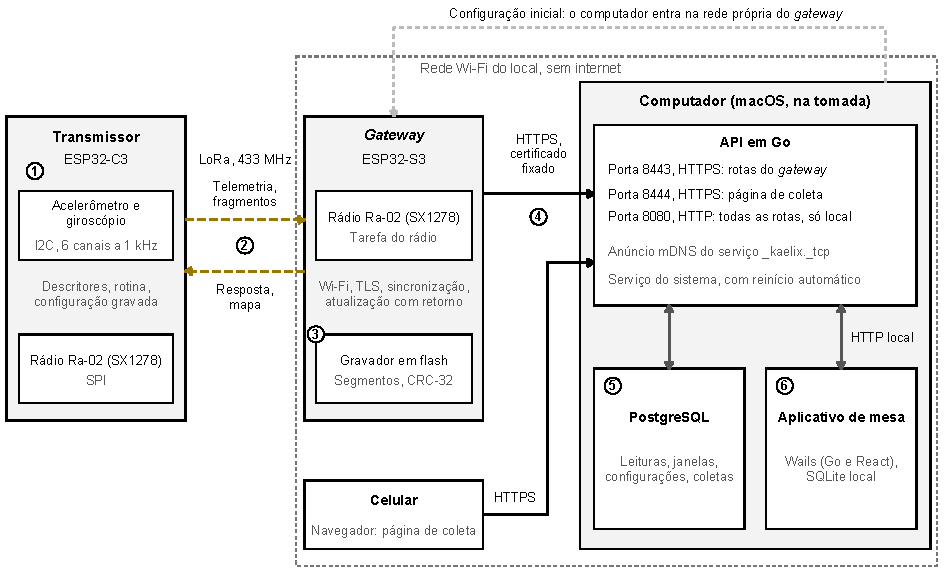
\includegraphics[width=\textwidth]{fig12_implantacao.pdf}
\fonte{elaborado pelo próprio autor.}
\legenda{os números indicam a ordem das etapas: medição no transmissor (1), envio pelo rádio (2), gravação na memória do \textit{gateway} (3), envio à API por HTTPS (4), gravação no banco (5) e consulta pelo aplicativo (6). Cada seta tem ao lado o nome do enlace. As tracejadas em amarelo-escuro são as do rádio LoRa, com a mesma cor do rádio nas Figuras~\ref{fig:sis-ciclo} e~\ref{fig:sis-configuracao}; as contínuas em preto são HTTPS pela rede Wi-Fi do local, e as em cinza, a comunicação dentro do computador.}
\end{figure}

Cada parte guarda o estado de que precisa para continuar funcionando quando a parte seguinte está fora do ar. O transmissor guarda a última configuração aceita e mede sem o \textit{gateway} (R2). O \textit{gateway} guarda as medições até a API confirmar o recebimento (R6). A API guarda a configuração desejada de cada dispositivo e a entrega ao \textit{gateway} na sincronização seguinte, a consulta que o \textit{gateway} faz à API a cada \SI{5}{\second}. O \textit{gateway}, por sua vez, repassa a configuração ao transmissor na próxima resposta pelo rádio.

O transmissor envia a janela de sinal bruto inteira, além dos indicadores (R7), e a janela ocupa o rádio por mais tempo que a telemetria. A telemetria de \num{71} bytes ocupa o rádio por \SI{411}{\milli\second}, e os \num{26} fragmentos de uma janela, por \SI{5,1}{\second}, sem contar os intervalos e os reenvios (seção~\ref{sec:fund-lora}). Com o sinal bruto no banco, a detecção pôde ser refeita com outra regra sobre as mesmas janelas, como nas análises posteriores (seção~\ref{sec:res-posteriores}).

A API atende em três portas, cada uma com um conjunto de rotas, os endereços de requisição que ela aceita. A porta \num{8080}, em HTTP, sem cifra, aceita todas as rotas, mas apenas em conexões do próprio computador, e serve ao aplicativo de mesa. A porta \num{8443}, em HTTPS, fica aberta à rede local e aceita apenas as rotas do \textit{gateway}. A porta \num{8444}, também em HTTPS, serve a página de coleta e só é aberta quando configurada.

O protocolo de rádio é definido num único arquivo de cabeçalho em C++, incluído na compilação dos dois \textit{firmwares}. Da mesma forma, a API e o aplicativo usam o mesmo pacote em Go, o pacote de contratos, para os formatos das mensagens e para as regras de validação da configuração (Quadro~\ref{quadro:sis-componentes}). Uma mudança no formato de um quadro de rádio é feita, assim, num único lugar e vale para os dois \textit{firmwares} a partir da compilação seguinte, e uma mudança numa mensagem vale para a API e para o aplicativo.

\begin{quadro}[!htb]
\centering\small
\caption{Componentes de \textit{software} do sistema}\label{quadro:sis-componentes}
\begin{tabular}{@{}>{\raggedright\arraybackslash}p{28mm}>{\raggedright\arraybackslash}p{50mm}r>{\raggedright\arraybackslash}p{46mm}@{}}
\toprule
Componente & Linguagem e bibliotecas & Linhas & Função \\
\midrule
\textit{Firmware} do transmissor & C++17 e C, Arduino-ESP32 2.0.17, RadioLib 7.7.1 & \sisLinhasTransmissor & aquisição, indicadores, telemetria, rajada, configuração e rotina \\
\addlinespace
\textit{Firmware} do \textit{gateway} & C++17, Arduino-ESP32 2.0.17, RadioLib 7.7.1, ArduinoJson 7.4.2, LittleFS & \sisLinhasGateway & recepção, gravação na \textit{flash}, entrega por HTTPS, configuração sem cabo e atualização \\
\addlinespace
Protocolo de rádio & C++17, cabeçalho único & \sisLinhasProtocolo & quadros, validação, perfis e tempos, compilado nos dois \textit{firmwares} \\
\addlinespace
Bibliotecas comuns & C++17 & \sisLinhasComum & CRC, códigos de estado e processamento de sinal \\
\addlinespace
API & Go 1.26.6, biblioteca padrão \texttt{net/http}, pgx 5.11.0 & \sisLinhasApi & ingestão idempotente, configuração, comandos, coletas e página de coleta \\
\addlinespace
Esquema do banco & SQL, PostgreSQL & \sisLinhasSql & cinco migrações numeradas \\
\addlinespace
Contratos & Go 1.26.0 & \sisLinhasContratos & formatos das mensagens e validação da configuração \\
\addlinespace
Aplicativo de mesa & Go 1.26.0 e Wails 2.13.0; React 19.3.0 e TypeScript 5.9.3 & \sisLinhasMesaGo\ e \sisLinhasMesaUi & pareamento, configuração, coletas, sinal e exportação \\
\bottomrule
\end{tabular}
\fonte{elaborado pelo próprio autor.}
\nota{linhas dos arquivos-fonte, com comentários e linhas em branco, sem os testes; no aplicativo, a primeira contagem é do processo em Go, e a segunda, da interface. SQL: linguagem de consulta estruturada.}
\end{quadro}

\section{Protocolo de rádio}\label{sec:sis-protocolo}

O protocolo de rádio da coleta, na versão 3, tem quatro tipos de quadro (Tabela~\ref{tab:sis-quadros}). Todo quadro começa pela versão e pelo tipo e termina num CRC de \num{16} bits, calculado sobre os bytes anteriores. O CRC usa o polinômio $x^{16} + x^{12} + x^{5} + 1$, do padrão CCITT, da antiga Comissão Consultiva Internacional de Telegrafia e Telefonia. Os campos de mais de um byte são gravados com o byte menos significativo primeiro, na ordem chamada \textit{little-endian}, e sem bytes de preenchimento entre os campos. O tamanho de cada estrutura em bytes é verificado na compilação, por uma asserção estática, e uma alteração acidental no formato impede a compilação. Os campos de cada quadro estão no Apêndice~\ref{ap:protocolo}.

\begin{table}[!htb]
\centering\small
\caption{Quadros do protocolo de rádio}\label{tab:sis-quadros}
\begin{tabular}{@{}>{\raggedright\arraybackslash}p{62mm}llrr@{}}
\toprule
Quadro & Destino & Canal & Bytes & Tempo no ar (ms) \\
\midrule
Telemetria & \textit{gateway} & controle & \num{71} & \num{411} \\
Resposta sem configuração & transmissor & controle & \num{22} & \num{206} \\
Resposta com configuração e seis horários de rotina & transmissor & controle & \num{75} & \num{432} \\
Fragmento completo & \textit{gateway} & rajada & \num{254} & \num{200} \\
Mapa da rajada & transmissor & rajada & \num{44} & \num{47} \\
\bottomrule
\end{tabular}
\fonte{elaborado pelo próprio autor.}
\nota{tempo no ar calculado pela Equação~\eqref{eq:fund-toa}, com o canal de controle em fator de espalhamento (SF) 9 e banda de \SI{125}{\kilo\hertz} e a rajada no perfil padrão, SF 7 e banda de \SI{250}{\kilo\hertz}. O fragmento completo leva \num{240} bytes de amostras e \num{14} bytes de cabeçalho e CRC.}
\end{table}

O enlace usa dois canais de rádio, o de controle e o da rajada. O canal de controle leva a telemetria e a resposta do \textit{gateway}, em \SI{433}{\mega\hertz}, com fator de espalhamento 9, banda de \SI{125}{\kilo\hertz}, taxa de codificação 4/5 e palavra de sincronismo \texttt{0x12}. Os parâmetros do canal de controle são constantes do \textit{firmware} e não fazem parte da configuração remota (R3). O canal da rajada leva os fragmentos da janela e o mapa da rajada, quadro em que o \textit{gateway} informa quais fragmentos recebeu. Ele usa um dos quatro perfis da Tabela~\ref{tab:sis-perfis}, escolhido na configuração do transmissor e informado na telemetria, e o \textit{gateway} passa ao perfil informado. O perfil padrão, com fator de espalhamento 7 e banda de \SI{250}{\kilo\hertz}, transmite a \SI{10,94}{kbit/s}, cerca de seis vezes a taxa do canal de controle.

\begin{table}[!htb]
\centering\small
\caption{Perfis da rajada}\label{tab:sis-perfis}
\begin{tabular}{@{}cccccc@{}}
\toprule
Código & SF & Banda (kHz) & Taxa (kbit/s) & Janela no ar (s) & Ciclo mínimo (s) \\
\midrule
0 & 9 & \num{125} & \num{1,76} & \num{32,1} & \num{36} \\
1 & 7 & \num{125} & \num{5,47} & \num{10,3} & \num{14} \\
2 (padrão) & 7 & \num{250} & \num{10,94} & \num{5,1} & \num{9} \\
3 & 7 & \num{500} & \num{21,88} & \num{2,6} & \num{7} \\
\bottomrule
\end{tabular}
\fonte{elaborado pelo próprio autor.}
\nota{SF: fator de espalhamento. Janela de \num{512} amostras em seis canais, dividida em \num{26} fragmentos. ``Janela no ar'' é a soma dos tempos no ar dos fragmentos, sem os intervalos e sem reenvios. ``Ciclo mínimo'' é o menor intervalo entre ciclos que a API aceita para essa janela, pela regra da seção~\ref{sec:sis-configuracao}.}
\end{table}

A taxa de todos os perfis fica abaixo da taxa do sinal contínuo, e por isso o transmissor envia janelas separadas por intervalos. Os seis canais a \SI{1}{\kilo\hertz}, com \num{16} bits por amostra, somam \SI{96}{kbit/s}, quase nove vezes a taxa do perfil padrão. Uma janela de \num{512} amostras dos seis canais tem \num{6144} bytes e é dividida em \num{26} fragmentos, \num{25} com \num{240} bytes de amostras e o último com \num{144}. No perfil 0, que usa os parâmetros do canal de controle, os \num{26} fragmentos ocupam o rádio por \SI{32,1}{\second}, e no perfil padrão, por \SI{5,1}{\second}. Um perfil de taxa maior ocupa o rádio por menos tempo, mas exige sinal mais forte no receptor \cite{semtech2015}. O alcance de cada perfil não foi medido.

A telemetria é enviada em todo ciclo, com ou sem janela. O número de sequência da telemetria cresce a cada ciclo, e a contagem de inicializações cresce a cada reinício do transmissor por perda de energia. Juntos, os dois números distinguem uma telemetria perdida, que deixa lacuna na sequência, de um reinício, que a faz voltar a zero (seção~\ref{sec:sis-transmissor}). Ao ligar, o transmissor não tem hora válida. A hora passa a valer quando uma resposta do \textit{gateway} a sincroniza, e um sinalizador da telemetria indica se a sincronização já ocorreu.

Num ciclo com janela, a telemetria, a resposta e os fragmentos ocupam o rádio em sequência, e a rajada só começa depois que o \textit{gateway} a autoriza (Figura~\ref{fig:sis-ciclo}). O transmissor lê a janela, o que leva \SI{512}{\milli\second} com \num{512} amostras, envia a telemetria no canal de controle e abre a recepção por até \SI{300}{\milli\second}. O \textit{gateway} responde \SI{20}{\milli\second} depois do fim da telemetria. A resposta confirma o número de sequência e leva a hora em tempo universal coordenado (UTC), a configuração desejada, quando a versão difere da relatada, e o comando pendente, quando há um. O \textit{gateway} só autoriza a rajada depois de reservar memória para a janela e conferir o número de fragmentos anunciado. Com a autorização, os dois passam ao perfil da rajada, e o transmissor envia o primeiro fragmento \SI{120}{\milli\second} depois e os seguintes com \SI{50}{\milli\second} entre eles. Os \SI{120}{\milli\second} dão ao \textit{gateway} tempo para trocar de perfil e passar a leitura à tarefa que a grava na \textit{flash} (seção~\ref{sec:sis-gravador}).

\begin{figure}[!htb]
\centering
\caption{Ciclo de medição com janela no perfil padrão da rajada}\label{fig:sis-ciclo}
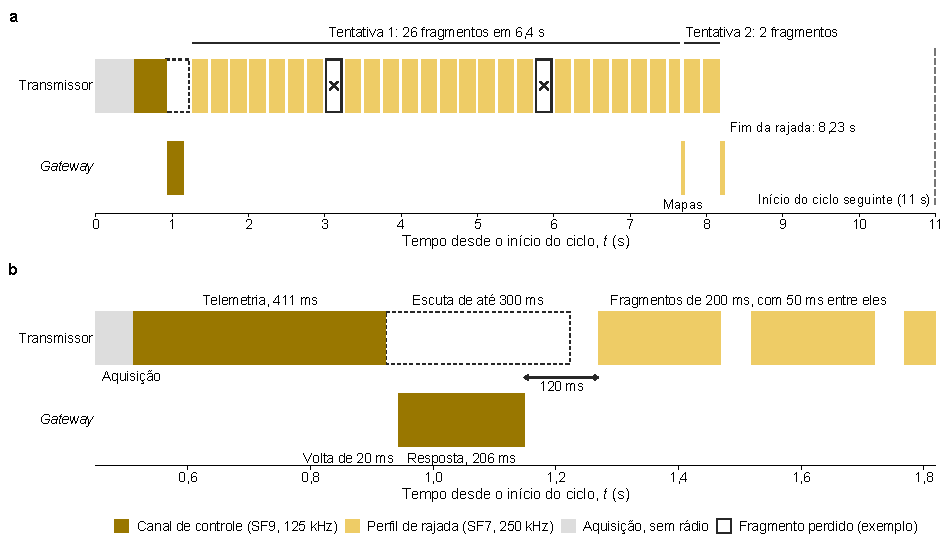
\includegraphics[width=\textwidth]{fig13_ciclo_radio.pdf}
\fonte{elaborado pelo próprio autor.}
\legenda{tempos calculados pela Equação~\eqref{eq:fund-toa}, para janela de \num{512} amostras em seis canais; os dois fragmentos perdidos são um exemplo. \textbf{a}, ciclo completo, com duas tentativas na rajada. \textbf{b}, início do ciclo: telemetria, escuta, resposta e primeiros fragmentos.}
\end{figure}

Ao fim de cada tentativa da rajada, o \textit{gateway} envia o mapa, com um bit por fragmento recebido, e o transmissor reenvia apenas os fragmentos ausentes (seção~\ref{sec:fund-blocos}). A tentativa termina depois de um silêncio de duas durações de fragmento mais \SI{100}{\milli\second}, e a rajada tem no máximo três tentativas, o envio inicial e dois reenvios. Uma janela incompleta depois da terceira tentativa é gravada com a lista dos fragmentos ausentes, e as amostras desses fragmentos chegam ao banco com valor zero. Quando nenhum fragmento chega, o \textit{gateway} não envia mapa, e o transmissor, sem o mapa, descarta a janela. No exemplo da Figura~\ref{fig:sis-ciclo}, com dois fragmentos perdidos na primeira tentativa, a rajada termina \SI{8,2}{\second} depois do início do ciclo, antes do ciclo seguinte, que começa em \SI{11}{\second}.

Um quadro corrompido no ar é descartado sem resposta. O circuito de rádio SX1278 descarta o quadro cujo CRC de rádio não confere, e o receptor confere o CRC do protocolo antes de decodificar o quadro aceito. O \textit{gateway} descarta também, sem responder, o quadro com versão ou tipo errados. Como a telemetria não é retransmitida e o \textit{gateway} só autoriza a rajada depois de recebê-la, uma telemetria perdida faz perder também a janela do ciclo. A perda fica registrada como lacuna no número de sequência.

\section{\textit{Firmware} do transmissor}\label{sec:sis-transmissor}

O transmissor usa um ESP32-C3 ligado ao módulo do acelerômetro e giroscópio pelo barramento I2C e ao rádio Ra-02, com o circuito SX1278, por uma interface serial periférica (SPI) (seção~\ref{sec:sistema}). O \textit{firmware} foi escrito em C++ com o \textit{framework} Arduino e compilado com o PlatformIO, num ambiente de compilação que inclui apenas os módulos do transmissor: o ciclo de medição, o acesso ao sensor, o acesso ao rádio, o cálculo dos indicadores e os temporizadores de vigilância (\textit{watchdog}). A imagem do \textit{firmware} da coleta, o arquivo binário gravado na placa, ocupou \sisRamTransmissorPct~\% da memória de acesso aleatório (RAM) disponível, ou \sisRamTransmissorBytes\ bytes, e \sisFlashTransmissorPct~\% do espaço de aplicação da \textit{flash}, ou \sisFlashTransmissorBytes\ de \sisFlashTransmissorTotal\ bytes. O transmissor não aloca memória dinamicamente, e a janela e os vetores de cálculo têm tamanho fixo, definido na compilação.

\subsection{Aquisição}

Na inicialização, o \textit{firmware} lê o registrador de identificação do sensor e aceita dois valores: \texttt{0x68}, do MPU-6050, e \texttt{0x74}, que ele associa ao MPU6515. A memória interna do sensor, em que o primeiro dado a entrar é o primeiro a sair (FIFO), tem \num{512} bytes no MPU6515 e \num{1024} bytes no MPU-6050. O módulo da coleta respondeu \texttt{0x74} (seção~\ref{sec:sistema}). Depois de escrever os registradores de configuração, o \textit{firmware} os lê de volta e interrompe a medição com código de erro se algum valor diferir do escrito.

O sensor amostra a \SI{1}{\kilo\hertz} e guarda as amostras na FIFO, que o \textit{firmware} esvazia pelo barramento I2C a \SI{400}{\kilo\hertz}, em lotes de até \num{10} amostras. O instante de cada amostra é dado, assim, pelo relógio do sensor, e uma pausa do processador não altera o espaçamento entre amostras enquanto a FIFO tiver espaço. Com seis canais, cada amostra ocupa \num{12} bytes, e a FIFO de \num{512} bytes comporta \num{42} amostras, ou \SI{42}{\milli\second} de sinal. Se a FIFO transbordar ou o barramento não responder, a aquisição termina com código de erro, e a janela não é enviada.

Depois da aquisição, o \textit{firmware} estima a taxa de amostragem da janela pelos carimbos de tempo da FIFO. Quando a taxa se afasta mais de \SI{2}{\percent} de \SI{1}{\kilo\hertz}, a telemetria informa o código de diagnóstico correspondente e os indicadores como não medidos, e a janela é enviada com a taxa estimada. Uma janela com amostra no limite da faixa do sensor recebe o sinalizador de saturação. A faixa do acelerômetro, a do giroscópio, o filtro interno e os canais são definidos pela configuração remota (seção~\ref{sec:sis-configuracao}).

\subsection{Ciclo, rotina e sono}

Cada ciclo começa num instante fixo, separado do início do anterior pelo intervalo da configuração, de \SI{11}{\second} por padrão. Quando a espera até o próximo ciclo passa de \SI{30}{\second}, o transmissor entra em sono profundo, com o rádio e o sensor desligados. Em esperas menores, apenas o rádio entra em modo de baixo consumo, e o processador e o sensor continuam ligados até o ciclo seguinte. Na coleta, com ciclos de \campoCicloUm\ e de \campoCicloDois~s, o transmissor não entrou em sono profundo, e o consumo não foi medido.

A rotina define até seis horários de medição, cada um com dias da semana, hora de início e hora de fim. Fora deles, o transmissor não mede e acorda a cada intervalo de consulta, de \SI{300}{\second} por padrão, para enviar uma telemetria sem medição, marcada por um sinalizador, e receber comandos. A rotina só é seguida depois que o transmissor recebe a hora do \textit{gateway}, e, sem hora sincronizada, ele mede em todos os ciclos.

Dois temporizadores de vigilância reiniciam o transmissor quando o ciclo para. O da tarefa tem prazo de \SI{6}{\second}, e o ligado ao relógio de tempo real (RTC) tem prazo de \SI{20}{\second} por ciclo, estendido durante a rajada.

A telemetria seguinte a um reinício permite saber se ele foi causado por perda de energia. O número de sequência fica na memória do RTC, que se mantém no sono profundo e num reinício por \textit{software} e se perde quando a alimentação é interrompida. Depois de uma interrupção, o estado guardado no RTC não passa na conferência do CRC, o número de sequência volta a zero e a contagem de inicializações, guardada na memória não volátil, cresce. A telemetria informa também a causa do último reinício, registrada pelo próprio ESP32-C3. Pelo número de sequência, pela contagem de inicializações e pela causa do reinício, foram identificados na coleta os reinícios por queda de tensão da bateria (seção~\ref{sec:res-aquisicao}).

\subsection{Indicadores e diagnóstico}

A cada janela, o transmissor calcula o valor eficaz nos três eixos de aceleração. No eixo Z, depois de remover a média da janela, calcula também a curtose, o fator de crista e a frequência dominante, o pico do espectro da velocidade entre \SI{10}{\hertz} e a metade da taxa de amostragem. A telemetria leva ainda a taxa de amostragem estimada e a temperatura interna do sensor. As funções de cálculo ficam numa biblioteca separada do acesso ao \textit{hardware} e são testadas no computador (seção~\ref{sec:sis-testes}). Os indicadores do transmissor não foram usados na avaliação da detecção, que usou os descritores calculados sobre as janelas exportadas (seção~\ref{sec:descritores}). Um detector Isolation Forest de \num{100} árvores, treinado em Python para o \textit{firmware} de bancada, foi convertido em código C++, mas esse código não entra na compilação do transmissor da coleta.

Cada função do \textit{firmware} devolve um código de estado, e o campo de diagnóstico da telemetria informa o primeiro erro do ciclo (Quadro~\ref{quadro:sis-diagnostico}). Quando a aquisição não se completa, os indicadores são enviados como valor não numérico (NaN), e a telemetria do ciclo é transmitida normalmente. Uma versão anterior do \textit{firmware} preenchia a janela com zeros em caso de erro, e os indicadores calculados sobre esses zeros seriam classificados como máquina sadia. O código de diagnóstico foi zero em \sisCampoDiagZero\ das \sisCampoTelemetrias\ telemetrias dos trechos analisados.

\begin{quadro}[!htb]
\centering\small
\caption{Códigos de diagnóstico da telemetria}\label{quadro:sis-diagnostico}
\begin{tabular}{@{}l>{\raggedright\arraybackslash}p{68mm}>{\raggedright\arraybackslash}p{60mm}@{}}
\toprule
Código & Condição & Efeito no ciclo \\
\midrule
\texttt{0x10} & sensor ausente no barramento & indicadores como NaN; sem janela \\
\texttt{0x11} & identificação diferente de \texttt{0x68} e de \texttt{0x74} & indicadores como NaN; sem janela \\
\texttt{0x15} & FIFO transbordada ou taxa estimada a mais de \SI{2}{\percent} de \SI{1}{\kilo\hertz} & sem janela, no primeiro caso; indicadores como NaN, no segundo \\
\texttt{0x16} & amostra em $\pm\num{32760}$, no limite da faixa & sinalizador de saturação; janela enviada \\
\texttt{0x17} & janela com valor constante & indicadores como NaN; janela enviada \\
\bottomrule
\end{tabular}
\fonte{elaborado pelo próprio autor.}
\nota{os erros de barramento (tempo-limite e ausência de resposta) têm códigos próprios e terminam a aquisição como no primeiro caso.}
\end{quadro}

\section{\textit{Firmware} do \textit{gateway}}\label{sec:sis-gateway}

O \textit{gateway} usa um ESP32-S3 com \SI{16}{MiB} de memória \textit{flash} e \SI{8}{MiB} de memória pseudoestática (PSRAM), ligado ao mesmo modelo de rádio do transmissor. Ele recebe as telemetrias e as janelas pelo rádio, grava as medições, entrega os dados à API e repassa ao transmissor a configuração e os comandos. A imagem da coleta, na versão 2.1.1, ocupou \sisRamGatewayPct~\% da RAM, ou \sisRamGatewayBytes\ bytes, e \sisFlashGatewayPct~\% do espaço de aplicação, ou \sisFlashGatewayBytes\ de \sisFlashGatewayTotal\ bytes.

\subsection{Tarefas e gravador}\label{sec:sis-gravador}

O trabalho do \textit{gateway} é dividido em três contextos de execução do FreeRTOS, o sistema operacional de tempo real incluído no \textit{framework} Arduino do ESP32. O laço principal atende o rádio e é o único a usar o barramento SPI, uma tarefa grava os registros na \textit{flash}, e outra, de prioridade menor, cuida da rede. O laço do rádio responde ao transmissor antes de gravar a telemetria e passa cada leitura e cada janela à tarefa de gravação por uma fila de \num{32} posições. Com essa divisão, um envio lento à API não atrasa a resposta pelo rádio, enviada \SI{20}{\milli\second} depois do fim da telemetria. Com a fila cheia, o registro é contado como descartado, e o número de descartes é informado na mensagem periódica de estado (\textit{heartbeat}) que o \textit{gateway} envia à API. A cada \SI{5}{\second}, o laço do rádio lê o registrador de versão do SX1278 para conferir que o rádio responde, e um temporizador de vigilância reinicia o \textit{gateway} se uma tarefa parar.

O gravador é a parte do \textit{firmware} que guarda as medições na \textit{flash} até a confirmação da API. Ele usa uma partição de \SI{9,88}{MiB}, formatada com o sistema de arquivos LittleFS (Figura~\ref{fig:sis-atualizacao}a), e escreve em segmentos de \SI{256}{KiB}. Cada registro tem um cabeçalho de \num{12} bytes, com tipo, tamanho e CRC de \num{32} bits, e passa a valer apenas depois de gravado e sincronizado com a \textit{flash}. Cada inicialização abre um segmento novo, e por isso um registro cortado por queda de energia só pode estar no fim de um segmento antigo. Ao encontrar, num segmento antigo, um registro incompleto ou com CRC errado, a tarefa de rede o conta como corrompido e passa a ler o segmento seguinte. Quando a escrita de um registro retorna erro, a tarefa de gravação tenta de novo até três vezes, e um registro não gravado é contado como descartado. A posição do último registro confirmado pela API também é gravada com CRC, a cada \num{16} confirmações.

O gravador comporta \num{1442} ciclos com janela padrão, o que corresponde a \SI{4,4}{\hour} de coleta com intervalo de \SI{11}{\second} e janela em todo ciclo. Cada ciclo ocupa \num{6460} bytes, \num{143} da leitura e \num{6317} da janela, com os cabeçalhos, e o gravador usa até \SI{90}{\percent} do sistema de arquivos. Com o gravador cheio, o segmento mais antigo é apagado, e o número de registros descartados é informado na mensagem de estado. A retenção do requisito R6 vale, portanto, dentro dessa capacidade.

A tarefa de rede lê o gravador a partir da última posição confirmada e envia à API as leituras em lotes de até oito e cada janela numa requisição própria. Cada leitura e cada janela leva o identificador do \textit{gateway}, o da sessão de inicialização, sorteado a cada inicialização, e um número de ordem crescente, atribuído pelo \textit{gateway}. A API grava cada registro uma única vez por esse trio, e por isso um reenvio depois de uma queda da rede ou da API não duplica dados (seção~\ref{sec:fund-entrega}). A tarefa só avança a posição confirmada quando a resposta da API indica cada registro enviado como gravado ou repetido. Quando a resposta indica erro permanente, como corpo inválido ou conflito de conteúdo, a tarefa descarta o registro. Nos demais erros, a tarefa repete o envio com espera crescente, de \SIrange{1}{30}{\second}, e, depois de três erros seguidos, procura a API de novo na rede.

O \textit{gateway} mantém também um histórico de eventos, uma sequência de linhas de texto que descrevem a sua operação, como a recepção de cada rajada. A memória do \textit{gateway} guarda até \num{64} linhas, que são enviadas à API, e a API mantém as \num{5000} linhas mais recentes de cada \textit{gateway}. A linha de cada rajada informa o número de fragmentos recebidos e a duração, e as rajadas analisadas na seção~\ref{sec:res-aquisicao} foram extraídas desse histórico (seção~\ref{sec:dados}).

\subsection{Rede e segurança}

O \textit{gateway} guarda até cinco redes Wi-Fi e conecta-se à de sinal mais forte. Ele localiza a API pelo anúncio que ela faz na rede local por resolução de nomes por difusão (mDNS), sem endereço de protocolo de internet (IP) gravado. Por isso, uma mudança no endereço do computador não exige regravar o \textit{gateway}.

A conexão com a API usa TLS, com um certificado próprio, gerado pela API na primeira execução, sem autoridade certificadora (seção~\ref{sec:fund-tls}). O \textit{gateway} compara o resumo SHA-256 do certificado recebido com o resumo gravado na configuração inicial e, se os dois diferirem, encerra a conexão antes de enviar a credencial (R8). A credencial é uma sequência aleatória de \num{43} caracteres (\textit{token}), enviada em cada requisição, e a API guarda apenas o resumo SHA-256 dela.

Sem rede conhecida por \SI{30}{\second}, o \textit{gateway} abre uma rede Wi-Fi própria, com nome formado pelos últimos quatro dígitos do endereço de controle de acesso ao meio (MAC), e oferece quatro rotas HTTP locais: informações do \textit{gateway}, lista das redes visíveis, configuração inicial e reinício. O assistente do aplicativo usa essa rede para enviar ao \textit{gateway} o identificador, o \textit{token}, uma chave de administração, o resumo do certificado e as redes Wi-Fi do local. Enquanto a rede própria está aberta, o \textit{gateway} continua a receber e a gravar as medições do rádio. Manter pressionado o botão de inicialização por \SI{10}{\second} apaga o pareamento, isto é, os dados recebidos na configuração inicial.

\subsection{Atualização sem cabo}

A \textit{flash} tem dois espaços de aplicação de \SI{3}{MiB}, e a imagem nova é gravada no espaço que não está em uso, sem apagar a que está em execução (Figura~\ref{fig:sis-atualizacao}a). O aplicativo envia a imagem à API, e a sincronização seguinte informa ao \textit{gateway} a versão, o tamanho, o resumo SHA-256 e o endereço de onde baixá-la. O \textit{gateway} baixa a imagem por HTTPS, confere o tamanho e o resumo e reinicia com ela. Uma imagem com tamanho ou resumo diferente é descartada, e o \textit{gateway} continua na versão atual.

\begin{figure}[!htb]
\centering
\caption{Partições da \textit{flash} do \textit{gateway} e etapas da atualização sem cabo}\label{fig:sis-atualizacao}
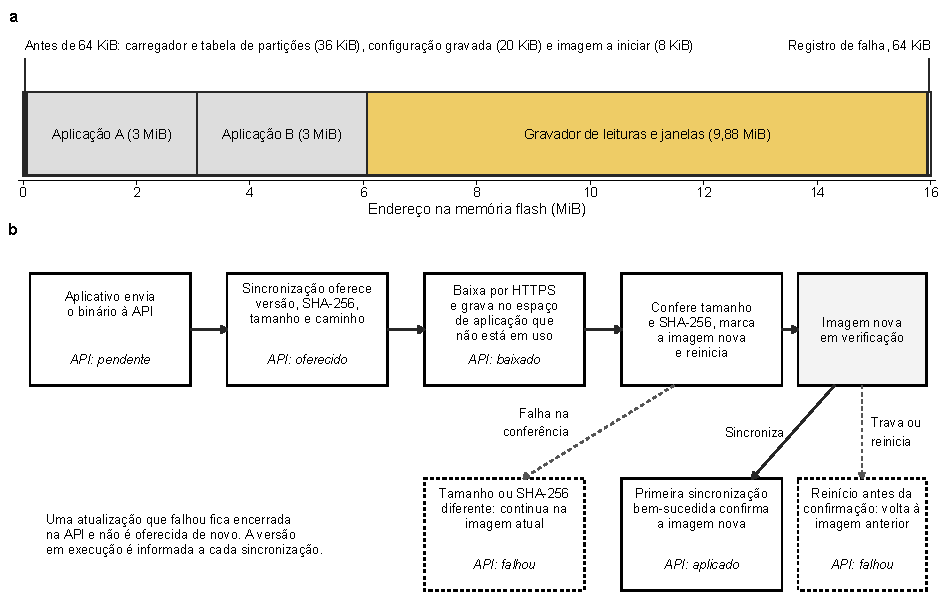
\includegraphics[width=\textwidth]{fig15_atualizacao.pdf}
\fonte{elaborado pelo próprio autor.}
\legenda{\textbf{a}, partições definidas na tabela do \textit{firmware}, em escala. \textbf{b}, etapas da atualização, com o estado registrado pela API em cada uma; as caixas tracejadas são as saídas sem sucesso.}
\end{figure}

A imagem nova fica em verificação até a primeira sincronização bem-sucedida com a API, que a confirma. Se o \textit{gateway} reiniciar antes da confirmação, o carregador de inicialização volta à imagem anterior, e a API registra a atualização como malsucedida (R9). Uma atualização malsucedida fica encerrada na API e não é oferecida de novo. A atualização sem cabo cobre apenas o \textit{gateway}, e o \textit{firmware} do transmissor é gravado pela porta de barramento serial universal (USB).

\section{Configuração remota e comandos}\label{sec:sis-configuracao}

A configuração do transmissor tem \num{14} campos (Quadro~\ref{quadro:sis-config}), e cada alteração recebe da API um número de versão. As faixas de cada campo e a regra do ciclo mínimo ficam no pacote de contratos, usado pela API e pelo aplicativo, e os dois recusam a mesma configuração pelo mesmo motivo. Pela regra do ciclo mínimo, a soma do tempo de aquisição, do tempo do canal de controle e do tempo da rajada, calculado pela Equação~\eqref{eq:fund-toa}, não pode ultrapassar o intervalo do ciclo. A configuração que o ultrapassa é recusada com a indicação do intervalo mínimo.

\begin{quadro}[!htb]
\centering\small
\caption{Campos da configuração do transmissor}\label{quadro:sis-config}
\begin{tabular}{@{}>{\raggedright\arraybackslash}p{50mm}>{\raggedright\arraybackslash}p{56mm}>{\raggedright\arraybackslash}p{44mm}@{}}
\toprule
Campo & Valores aceitos & Padrão \\
\midrule
Intervalo do ciclo & \SIrange{1}{3600}{\second} & \SI{11}{\second} \\
Amostras por canal & \num{256} a \num{4096}, em potências de 2 & \num{512} \\
Canais & combinação dos seis, com o eixo Z & os seis \\
Faixa do acelerômetro & $\pm\SI{2}{g}$ a $\pm\SI{16}{g}$ & $\pm\SI{4}{g}$ \\
Faixa do giroscópio & $\pm\SI{250}{\degree\per\second}$ a $\pm\SI{2000}{\degree\per\second}$ & $\pm\SI{250}{\degree\per\second}$ \\
Filtro interno do sensor & códigos 0 a 6 & 1, banda de \SI{184}{\hertz} \\
Potência de transmissão & \SIrange{2}{17}{dBm} & \SI{10}{dBm} \\
Perfil da rajada & 0 a 3 (Tabela~\ref{tab:sis-perfis}) & 2 \\
Janela a cada $N$ ciclos & 0 a \num{255}; 0 desliga o sinal bruto & 1 \\
Prazo de perda do enlace & \SIrange{60}{86400}{\second} & \SI{900}{\second} \\
Intervalo de consulta fora da rotina & \SIrange{60}{3600}{\second} & \SI{300}{\second} \\
Fuso horário da rotina & \SIrange{-720}{840}{\minute} & \SI{-180}{\minute} \\
Rotina & até seis horários de medição, com dias e horas & vazia, sempre ligado \\
Versão & \num{1} a \num{65535}, atribuída pela API & 0, configuração de fábrica \\
\bottomrule
\end{tabular}
\fonte{elaborado pelo próprio autor.}
\end{quadro}

Uma configuração nova passa por três estados na API, pendente, enviada e aplicada, e só é marcada como aplicada quando a telemetria do transmissor informa a versão nova (Figura~\ref{fig:sis-configuracao}). O aplicativo grava a configuração na API, que lhe atribui uma versão e a marca como pendente. A cada sincronização, o \textit{gateway} recebe da API as configurações e os comandos ainda não confirmados e os guarda numa tabela de até oito transmissores, na memória não volátil. Na telemetria seguinte daquele transmissor, a resposta leva a configuração, e a sincronização seguinte informa à API que ela foi enviada pelo rádio. O \textit{gateway} repete a configuração em cada resposta enquanto a versão relatada na telemetria for outra. A API marca a configuração como aplicada quando grava uma leitura com a versão nova (R4).

\begin{figure}[!htb]
\centering
\caption{Sequência de uma configuração nova do transmissor}\label{fig:sis-configuracao}
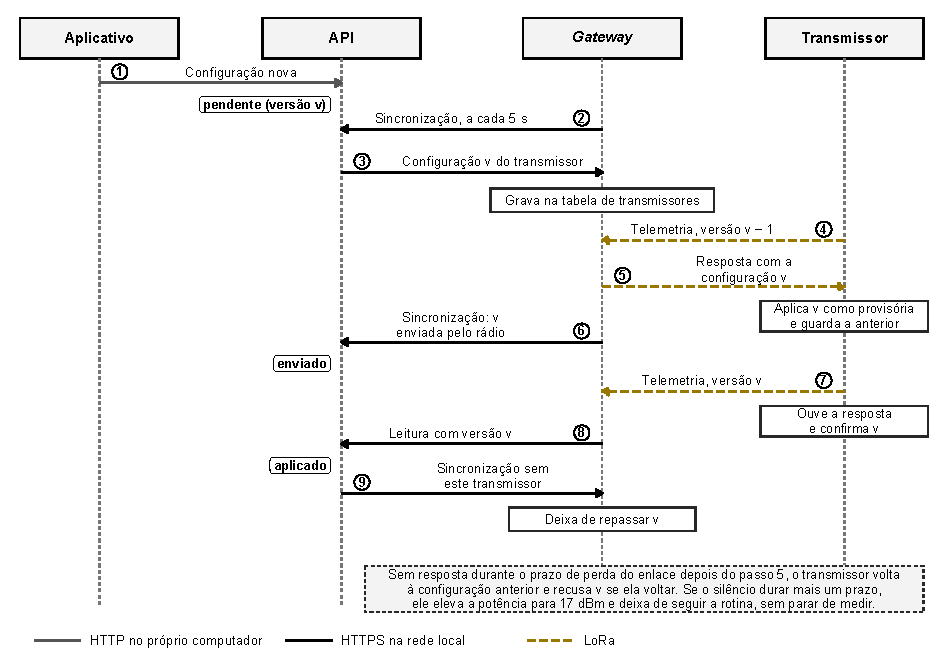
\includegraphics[width=\textwidth]{fig14_configuracao.pdf}
\fonte{elaborado pelo próprio autor.}
\legenda{os números indicam a ordem das mensagens, e os rótulos em negrito são os estados que a API registra para a configuração. $v$: versão da configuração nova.}
\end{figure}

O transmissor aplica a configuração nova como provisória e guarda a anterior na memória não volátil. Se não ouvir o \textit{gateway} durante o prazo de perda do enlace, de \SI{900}{\second} por padrão, ele volta à configuração anterior, que recebe um prazo novo, e recusa a versão revertida se ela for oferecida de novo (R5). Quando o prazo se esgota sem configuração provisória, o transmissor eleva a potência para \SI{17}{dBm} e deixa de seguir a rotina, sem parar de medir. Ao ouvir o \textit{gateway} de novo, ele volta à potência e à rotina da configuração.

O aplicativo envia ao transmissor três comandos, o de reinício, o de restauração da configuração de fábrica e o de captura de uma janela fora da rotina. Cada comando recebe um número crescente por transmissor, e a telemetria devolve o número do último comando executado. Ao registrar uma restauração de fábrica, a API troca também a configuração desejada pelos valores padrão, com versão nova, para que a configuração antiga não volte na sincronização seguinte.

O \textit{gateway} tem configuração própria, com as redes Wi-Fi, o intervalo da mensagem de estado (\SI{30}{\second}), o intervalo da sincronização (\SI{5}{\second}), a opção de abrir a rede própria quando nenhuma rede conhecida está ao alcance e a potência da resposta pelo rádio (\SI{17}{dBm}). As senhas de Wi-Fi ficam cifradas no banco e são enviadas ao \textit{gateway} apenas quando a versão da configuração do \textit{gateway} muda.

\section{API, banco de dados e aplicativo}\label{sec:sis-api}

A API foi escrita em Go, com a biblioteca padrão para o HTTP, e grava os dados em PostgreSQL. No computador da coleta, ela é executada como serviço do sistema operacional, que a reinicia se o processo terminar. O esquema do banco tem \num{16} tabelas (Quadro~\ref{quadro:sis-banco}), criadas por cinco migrações, alterações do esquema numeradas em ordem e aplicadas numa única transação. A tabela de leituras guarda a telemetria inteira, e a de janelas guarda o sinal bruto, como inteiros de \num{16} bits intercalados por canal, com a lista de fragmentos ausentes. A API não apaga leituras, janelas nem coletas.

\begin{quadro}[!htb]
\centering\small
\caption{Tabelas do banco de dados da API}\label{quadro:sis-banco}
\begin{tabular}{@{}>{\raggedright\arraybackslash}p{36mm}c>{\raggedright\arraybackslash}p{96mm}@{}}
\toprule
Grupo & Tabelas & Conteúdo \\
\midrule
Usuários & 2 & contas e sessões de usuário do aplicativo \\
\addlinespace
\textit{Gateways} & 7 & cadastro, sessões de inicialização, mensagens de estado, histórico de eventos, configuração e atualizações \\
\addlinespace
Transmissores e máquinas & 4 & cadastro dos transmissores e das máquinas, configuração desejada e relatada, comandos \\
\addlinespace
Medições & 2 & leituras e janelas de sinal bruto \\
\addlinespace
Coletas & 1 & intervalos de coleta com nome e condição da máquina \\
\bottomrule
\end{tabular}
\fonte{elaborado pelo próprio autor.}
\nota{uma das tabelas dos \textit{gateways} guarda as mensagens de estado no formato anterior ao atual.}
\end{quadro}

As rotas da API se dividem pelo cliente, o \textit{gateway} ou o aplicativo. As rotas do \textit{gateway} exigem o \textit{token} do próprio \textit{gateway}, e o identificador informado no corpo da requisição tem de coincidir com o da credencial. Elas recebem leituras, janelas, mensagens de estado e o histórico de eventos, atendem à sincronização e entregam a imagem de \textit{firmware}. As rotas do aplicativo exigem sessão de usuário e cobrem a configuração, os comandos, as janelas, as coletas, o envio de \textit{firmware} e o resumo do certificado, usado na configuração inicial do \textit{gateway}. A senha de cada usuário é guardada pela função bcrypt, própria para o resumo de senhas, e cada endereço IP tem no máximo dez tentativas de entrada por minuto.

A gravação de leituras e de janelas é idempotente, isto é, um reenvio não cria registro novo. A tabela de leituras e a de janelas têm restrição de unicidade sobre o trio formado pelo \textit{gateway}, pela sessão de inicialização e pelo número de ordem. Um lote repetido recebe a mesma confirmação, com o estado de repetido, e não gera linha nova. Um registro com o mesmo trio e conteúdo diferente é recusado como conflito, e o lote inteiro é desfeito.

Antes de gravar, a API confere o formato de cada requisição. Ela recusa o corpo com campo desconhecido ou chave repetida, o lote com mais de oito leituras e a janela cujo tamanho difere do produto do número de amostras pelo número de canais e por dois bytes. O corpo de uma janela é limitado a \SI{128}{KiB}. Ao gravar uma janela, a API calcula o resumo SHA-256 das amostras e o guarda com ela. Com esse resumo, calculado depois da recepção, é possível conferir a cópia das amostras do banco para os dados exportados (seção~\ref{sec:dados}), mas não a transmissão pelo rádio, conferida pelo CRC de cada fragmento.

As senhas de Wi-Fi são cifradas pelo padrão de cifra avançada (AES) no modo de contador com autenticação de Galois (GCM), com chave de \num{256} bits guardada num arquivo que apenas o usuário do serviço pode ler (seção~\ref{sec:fund-tls}). A chave e o certificado TLS, com chave de curva elíptica P-256, são gerados na primeira execução da API.

O aplicativo de mesa foi feito com Wails, que une um processo em Go a uma interface em React e TypeScript, e se comunica com a API pela porta local. A interface tem nove telas: monitoramento, motores, \textit{gateways}, transmissores, coletas, sinal, eventos, configurações e painel geral (Apêndice~\ref{ap:telas}). Por elas, o operador pareia e acompanha o \textit{gateway}, edita a configuração e a rotina do transmissor, envia comandos, inicia e encerra coletas e vê o resumo das perdas e o sinal de cada janela. A exportação de uma coleta gera tabelas em valores separados por vírgula (CSV), uma para as leituras, uma para a lista de janelas e uma para cada janela, com as amostras em unidades físicas e nos valores brutos do sensor. Os dados analisados neste trabalho não passaram por essa exportação. Eles foram lidos do banco em modo somente leitura por outro programa, e o resumo de cada janela foi conferido nessa leitura (seção~\ref{sec:dados}).

A página de coleta, servida pela API e aberta no celular, permite operar a coleta sem voltar ao computador (Figura~\ref{fig:sis-pagina-coleta}). Ela fica embutida no programa da API e exige a mesma conta do aplicativo. Pela página, o operador inicia e encerra coletas, muda o intervalo do ciclo do transmissor e acompanha o estado do \textit{gateway} e do transmissor e as últimas leituras, atualizadas a cada \SI{5}{\second}. Durante uma coleta, a página mostra também a duração, o número de leituras recebidas e perdidas, o número de janelas completas e a RSSI média e a menor RSSI do período.

\begin{figure}[!htb]
\centering
\caption{Página de coleta no celular, durante a coleta em campo}\label{fig:sis-pagina-coleta}
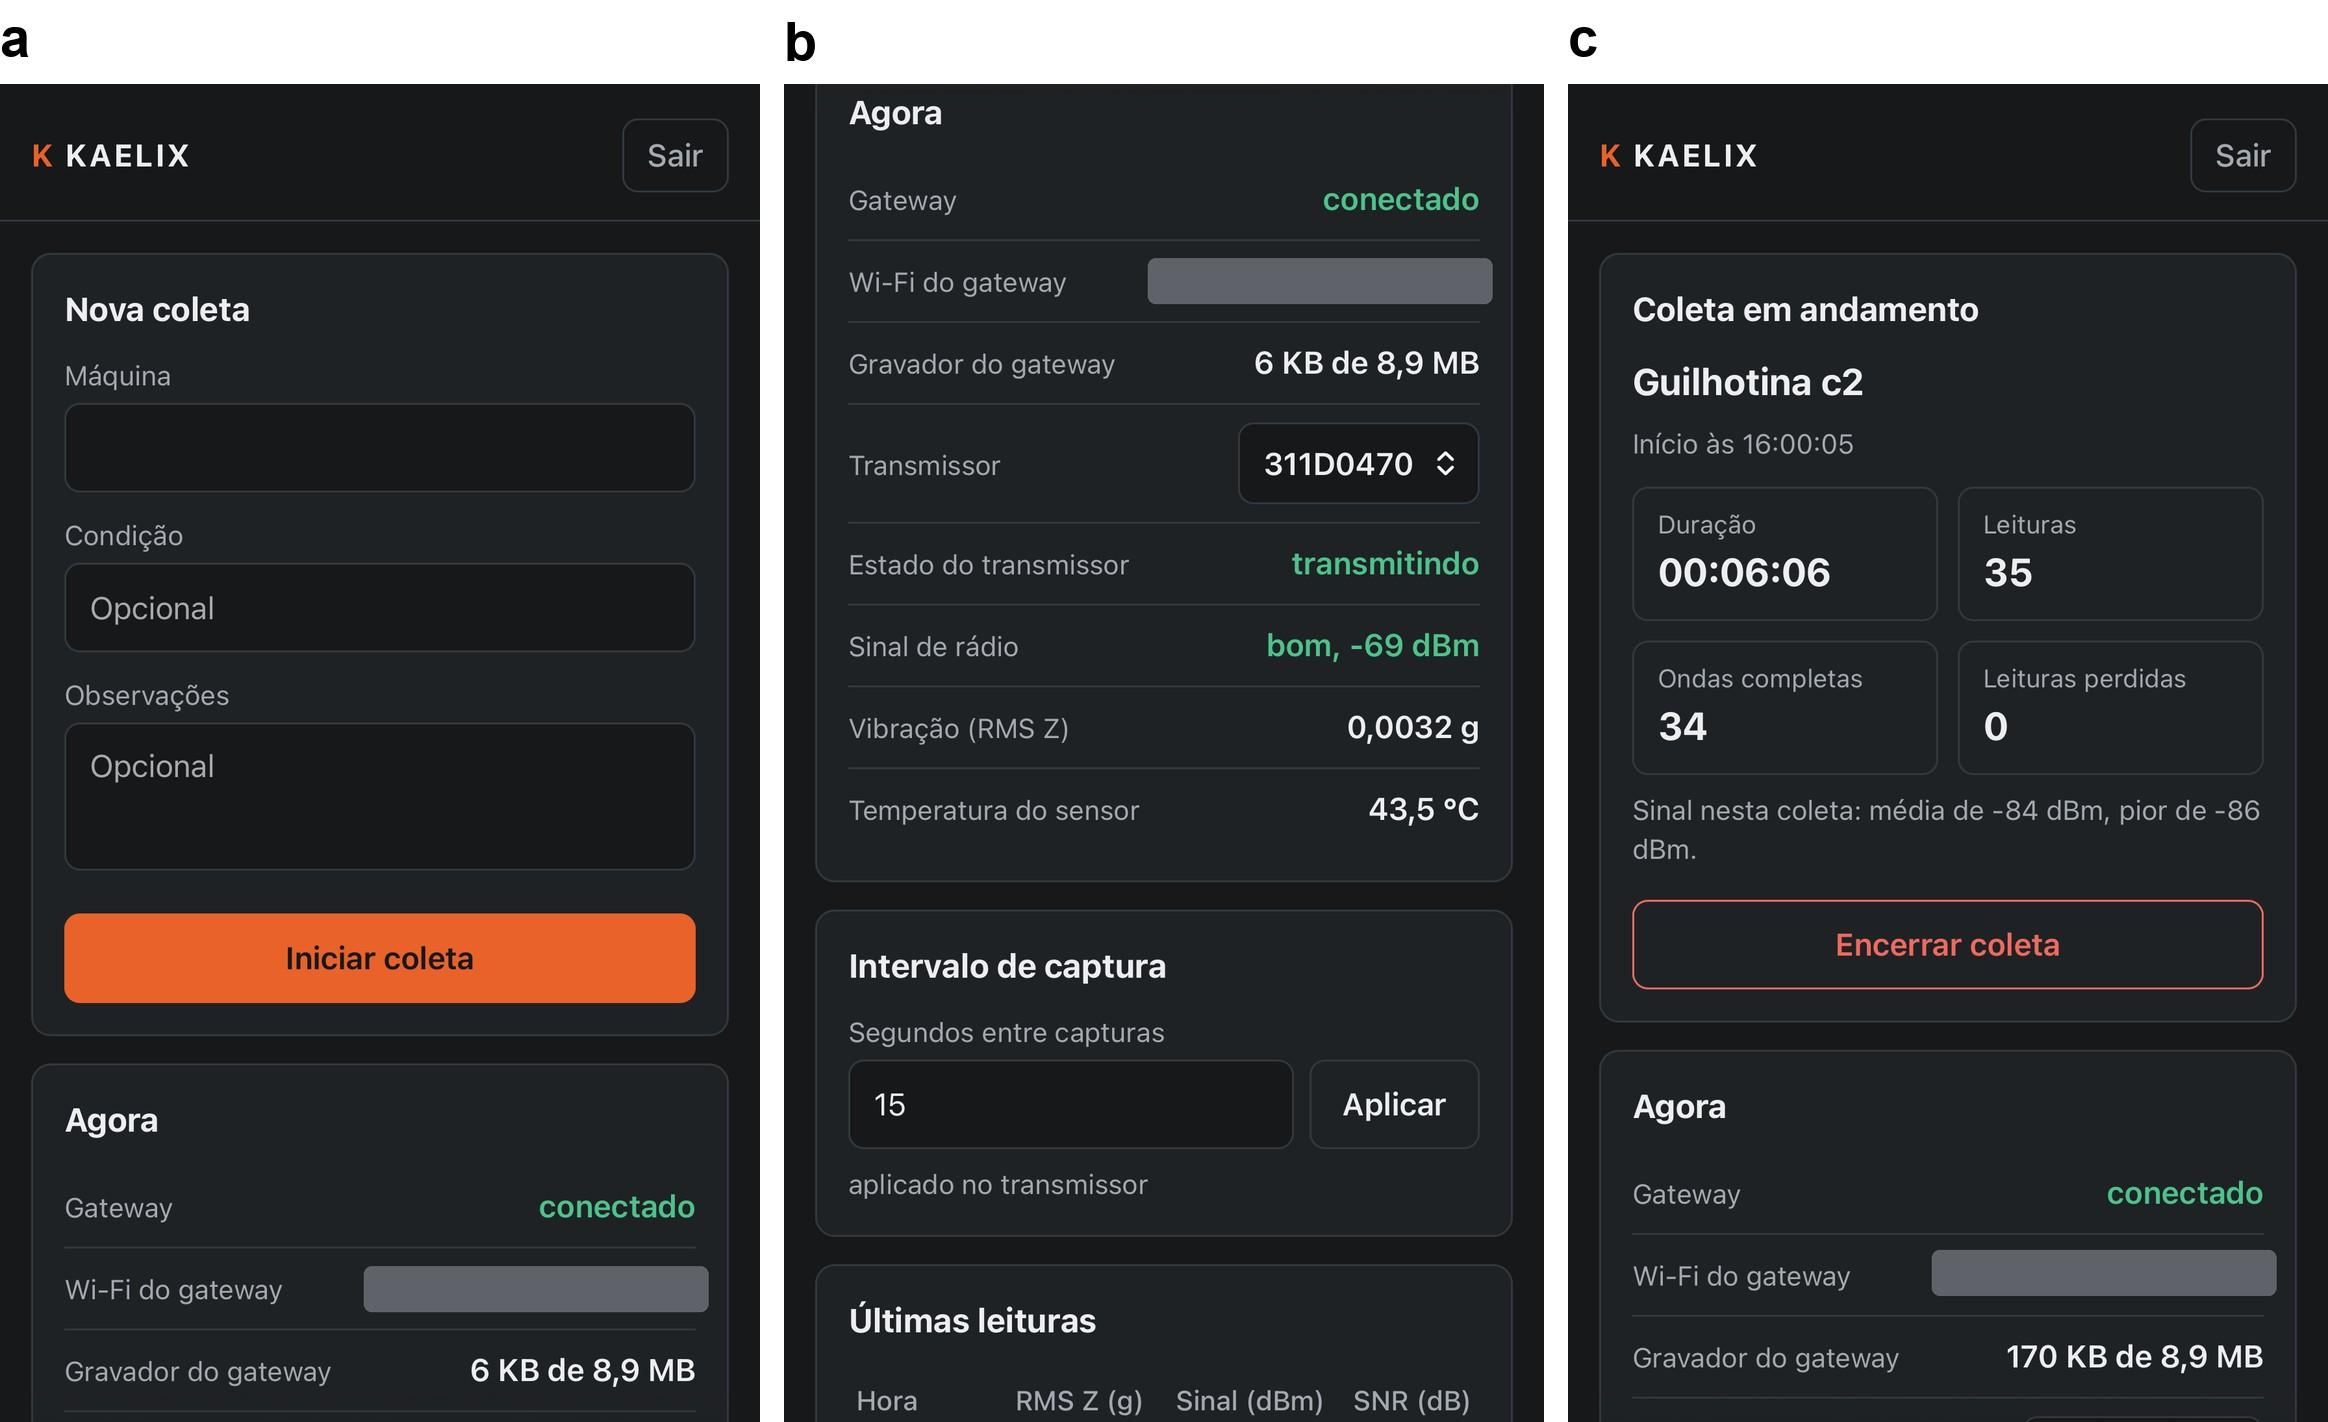
\includegraphics[width=\textwidth]{campo/fig17_pagina_coleta.jpg}
\fonte{elaborado pelo próprio autor.}
\legenda{\textbf{a}, início de uma coleta e estado do \textit{gateway}. \textbf{b}, estado do transmissor, intervalo do ciclo, chamado de intervalo de captura na página, e últimas leituras. \textbf{c}, segunda rodada da guilhotina em andamento; a captura de tela foi feita antes da chegada da última janela da rodada, e por isso a página mostra 34 ondas completas para 35 leituras. ``Ondas completas'' é o número de janelas de sinal bruto recebidas inteiras. Capturas de tela de 2 de novembro de 2026, sem a barra do navegador; o nome da rede Wi-Fi do local foi coberto por um retângulo cinza.}
\end{figure}

\section{Verificação}\label{sec:sis-verificacao}

O sistema foi verificado por quatro meios: uma norma de codificação, uma análise de modos de falha, testes automatizados no computador e ensaios de ponta a ponta no \textit{hardware} (seção~\ref{sec:fund-verificacao}). A norma e a análise de modos de falha foram escritas para o \textit{firmware} de bancada, versão anterior em que o transmissor enviava apenas os indicadores, sem a janela de sinal bruto. Os testes e os ensaios cobrem a versão da coleta.

\subsection{Norma de codificação}\label{sec:sis-norma}

O \textit{firmware} foi escrito segundo uma norma de codificação própria, com \num{41} regras em \num{14} áreas (Tabela~\ref{tab:sis-norma}). As regras foram selecionadas da MISRA C++:2008 \cite{misra2008}, que tem \num{228} regras, do padrão de codificação em C++ do programa Joint Strike Fighter \cite{jsf2005}, que tem \num{221}, e das dez regras de \citeonline{holzmann2006} para código crítico. Uma regra entrou na norma quando foi possível dizer qual falha do dispositivo ela impede e como a sua violação é detectada: pelo compilador, por análise estática, por teste ou por revisão. A norma lista \num{14} desvios aceitos, cada um com a justificativa.

\begin{table}[!htb]
\centering\small
\caption{Áreas da norma de codificação}\label{tab:sis-norma}
\begin{tabular}{@{}llc@{}}
\toprule
Prefixo & Assunto & Regras \\
\midrule
NC-ARQ & dependência entre camadas & 4 \\
NC-MEM & política de memória & 3 \\
NC-FLX & fluxo de controle: laços, recursão e limites & 4 \\
NC-ERR & tratamento e propagação de erro & 5 \\
NC-CTR & validação de parâmetros e contratos & 3 \\
NC-INI & inicialização de variáveis & 2 \\
NC-CNV & tipos e conversões & 3 \\
NC-FPU & ponto flutuante & 4 \\
NC-CST & constantes e uso de \texttt{const} & 2 \\
NC-ESC & escopo e visibilidade & 2 \\
NC-NOM & nomes & 3 \\
NC-HDR & arquivos de cabeçalho e inclusão & 2 \\
NC-COM & comentários & 2 \\
NC-BLD & compilação e verificação & 2 \\
\midrule
Total & & 41 \\
\bottomrule
\end{tabular}
\fonte{elaborado pelo próprio autor.}
\end{table}

Segundo a própria norma, as \num{41} regras servem ao requisito de que o dispositivo nunca afirme o que não mediu. As regras de tratamento de erro aplicam esse requisito diretamente: o valor não medido é NaN, nunca zero; todo caminho de erro produz o estado desconhecido; e uma função que termina com erro não escreve no seu parâmetro de saída.

A norma também proíbe alocação dinâmica de memória e recursão e exige que todo laço tenha um limite conhecido antes de começar. Com essas restrições, o tempo e a memória de cada ciclo podem ser calculados antes da execução.

Cada regra tem um meio de verificação atribuído. O compilador detecta o retorno de função não consumido, a conversão com perda de informação e a igualdade entre números de ponto flutuante, e asserções estáticas verificam na compilação o dimensionamento dos vetores e o formato dos quadros. Os testes no computador verificam as guardas de contrato, as verificações de pré-condição no início das funções. A revisão humana cobre o argumento do limite de cada laço e a classificação dos erros. O repositório do \textit{firmware} tem um \textit{script} que executa as ferramentas de análise estática clang-tidy e cppcheck para as regras de conversão, de nomes e de alocação. Não há registro de execução desse \textit{script}, e as duas ferramentas não estavam instaladas no computador de desenvolvimento em 7 de novembro de 2026.

A conformidade da versão da coleta com a norma tem três limites conhecidos. A regra NC-BLD-01 exige compilação com todos os avisos ativados e tratados como erro, e nenhum ambiente do PlatformIO, ferramenta que compila o \textit{firmware} das placas e executa os testes, ativa essas opções. A norma foi escrita em setembro de 2026 para o \textit{firmware} de bancada, antes do transmissor e do \textit{gateway} da coleta. O transmissor não aloca memória dinamicamente, mas o \textit{gateway} aloca, na fila de gravação, no gerenciador de redes Wi-Fi e na reserva da janela recebida, contra a regra NC-MEM-01, e esse uso não consta da lista de desvios.

\subsection{Análise de modos de falha}\label{sec:sis-falhas}

A análise de modos de falha e efeitos (FMEA) do \textit{firmware} de bancada listou \num{36} modos de falha em sete grupos: aquisição, temperatura, rádio, energia, execução, sono e telemetria. Cada modo recebeu uma classe de severidade, de S0 a S3, e uma classe de detectabilidade: D-A, quando o dispositivo detecta e informa a falha; D-B, quando o receptor consegue inferi-la com os dados que já recebe; e D-C, quando nenhum dos dois consegue detectá-la (seção~\ref{sec:fund-fmea}). A classe S3 é a do dado inválido aceito como válido, porque ele leva a uma decisão de manutenção errada sem nenhum sinal de erro. O Quadro~\ref{quadro:sis-falhas} mostra o mecanismo de detecção, na versão da coleta, de cada modo que continua aplicável à montagem sem termistor, sem medição de tensão da bateria e sem detector embarcado.

\begin{quadro}[!htb]
\centering\small
\caption{Modos de falha da FMEA na versão da coleta}\label{quadro:sis-falhas}
\begin{tabular}{@{}>{\raggedright\arraybackslash}p{44mm}>{\raggedright\arraybackslash}p{72mm}>{\raggedright\arraybackslash}p{34mm}@{}}
\toprule
Modo de falha & Mecanismo na versão da coleta & Quem detecta \\
\midrule
Sensor ausente ou que para no meio da janela (FM-01, FM-02) & tempo-limite ao ler a FIFO, código de erro no diagnóstico e indicadores como NaN & transmissor \\
\addlinespace
Valor saturado ou constante (FM-04) & sinalizador de saturação; código de sensor congelado para a janela constante & transmissor \\
\addlinespace
Sensor solto da máquina (FM-05) & nenhum & ninguém \\
\addlinespace
Telemetria perdida no ar (FM-11) & lacuna no número de sequência & API e operador \\
\addlinespace
Quadro corrompido (FM-13) & CRC do rádio e CRC do protocolo & \textit{gateway}, que descarta \\
\addlinespace
Queda de tensão (FM-15) & causa do reinício na telemetria seguinte; a tensão não é medida & transmissor, depois do reinício \\
\addlinespace
Travamento do \textit{firmware} (FM-17) & temporizadores de vigilância no transmissor e no \textit{gateway} & dispositivo, que reinicia \\
\addlinespace
Estado retido corrompido (FM-33) & CRC do estado guardado na memória do RTC & transmissor \\
\addlinespace
Causa do reinício não informada (FM-34) & causa do último reinício na telemetria e na mensagem de estado & transmissor e \textit{gateway} \\
\addlinespace
Desvio da taxa de amostragem (FM-35) & amostragem pelo relógio do sensor; código de diagnóstico e indicadores como NaN acima de \SI{2}{\percent} & transmissor \\
\addlinespace
Falta de hora no dispositivo (FM-36) & hora UTC sincronizada pela resposta do \textit{gateway}, com sinalizador & transmissor \\
\bottomrule
\end{tabular}
\fonte{elaborado pelo próprio autor.}
\nota{os modos de termistor, de carga da bateria e do detector embarcado ficaram fora do quadro, porque esses componentes não fazem parte da montagem da coleta.}
\end{quadro}

A FMEA não foi refeita para o \textit{gateway}. Os modos novos da montagem de campo, como a queda da API, um erro de gravação na \textit{flash} ou uma imagem de \textit{firmware} que não inicia, estão cobertos pelos requisitos R6 e R9, mas não receberam classe de severidade nem de detectabilidade.

\subsection{Testes automatizados}\label{sec:sis-testes}

As funções que não dependem do \textit{hardware} são testadas no computador. O \textit{firmware} tem \sisTestesSuites\ suítes de teste em C++, executadas pelo PlatformIO com o \textit{framework} de testes Unity (Tabela~\ref{tab:sis-testes}). Em 7 de novembro de 2026, os \sisTestesCasos\ casos passaram, em \sisTestesDuracao~s. As suítes foram executadas no modo de desenvolvimento, o mesmo em que os \textit{firmwares} da coleta foram compilados. No modo de desenvolvimento, uma pré-condição violada encerra o programa, e os testes que conferem esse encerramento executam a chamada num processo separado, para que a suíte continue.

O código testado é o mesmo dos \textit{firmwares} da coleta. O transmissor foi compilado às \sisCompilaTransmissor\ e o \textit{gateway}, às \sisCompilaGateway\ de 2 de novembro de 2026, e o código-fonte dos dois \textit{firmwares} não foi modificado depois dessas compilações.

\begin{table}[!htb]
\centering\small
\caption{Suítes de teste do \textit{firmware}}\label{tab:sis-testes}
\begin{tabular}{@{}>{\raggedright\arraybackslash}p{40mm}cc>{\raggedright\arraybackslash}p{78mm}@{}}
\toprule
Suíte & Casos & Coleta & O que cobre \\
\midrule
Protocolo de rádio & \sisCasosProtocol & sim & quadros da versão 3, configuração, rotina, tempo no ar, perda do enlace e retorno da configuração \\
Conversão no \textit{gateway} & \sisCasosGatewayVThree & sim & conversão para o formato da API, tabela de transmissores e remontagem da janela com reenvios \\
Gravador & \sisCasosSpool & sim & ordem dos registros, reinício, queda de energia no meio de um registro, capacidade e confirmação \\
Histórico de eventos & \sisCasosRemoteLogs & sim & envio das linhas à API \\
CRC de \num{16} bits & \sisCasosCrcSixteen & sim & CRC dos quadros e do estado retido \\
Processamento de sinal & \sisCasosSignalProcessing & sim & valor eficaz, curtose, fator de crista e frequência dominante \\
Indicadores de vibração & \sisCasosVibration & sim & indicadores sobre a janela do sensor, janela constante e valor não finito \\
Entrega na bancada & \sisCasosGatewayDelivery & não & confirmação dos lotes no receptor do \textit{firmware} de bancada \\
Pacote da bancada & \sisCasosPacketDecode & não & pacote do \textit{firmware} de bancada \\
Detector embarcado & \sisCasosIsolationForest & não & Isolation Forest convertido em C++, fora da compilação do transmissor \\
Termistor & \sisCasosThermistor & não & termistor, fora da montagem da coleta \\
\midrule
Total & \sisTestesCasos & & \\
\bottomrule
\end{tabular}
\fonte{elaborado pelo próprio autor.}
\nota{``Coleta'' indica se o código testado é compilado nos \textit{firmwares} usados na coleta.}
\end{table}

Sete suítes, com \sisTestesCampoCasos\ casos, testam código compilado nos \textit{firmwares} da coleta. O gravador do \textit{gateway} usa as funções de arquivo da biblioteca padrão do C, e o mesmo código é executado sobre o LittleFS na placa e sobre o disco do computador nos testes. Assim, os testes simulam o reinício do \textit{gateway} e a queda de energia no meio de um registro sem o \textit{hardware}. A biblioteca de processamento de sinal não inclui cabeçalhos do Arduino e também é compilada no computador. O acesso ao sensor e ao rádio no transmissor e o laço do rádio e a tarefa de rede no \textit{gateway} não têm teste no computador.

A API, o aplicativo e o pacote de contratos têm \sisGoFuncoes\ funções de teste em Go, em \sisGoArquivos\ arquivos: \sisGoFuncoesApi\ da API, \sisGoFuncoesMesa\ do aplicativo e \sisGoFuncoesContratos\ dos contratos. Os testes de contrato conferem as mensagens contra exemplos gerados pelo \textit{firmware}. Os testes da API cobrem a idempotência e o conflito, os limites de corpo, as janelas, a sincronização, o ciclo de vida dos comandos e das atualizações e a recusa das rotas do aplicativo na porta do \textit{gateway}. Os testes da API que usam banco são executados contra um PostgreSQL descartável, criado por um \textit{script} do repositório apenas para o teste, e são pulados quando o banco não está disponível. O detector de condições de corrida do Go fica ativado nesses testes e acusa o acesso simultâneo de duas rotinas à mesma variável sem sincronização. A interface em React não tem teste, e nem o repositório do \textit{firmware} nem o da API e do aplicativo têm integração contínua, a execução automática dos testes a cada alteração do código.

\subsection{Ensaios de ponta a ponta}\label{sec:sis-ensaios}

Na madrugada e na manhã de 2 de novembro de 2026, antes da coleta, o sistema foi ensaiado na bancada com o mesmo transmissor e o mesmo \textit{gateway}, o protocolo da versão 3 e a API num banco de teste. O banco de teste recebeu \sisBancoLeituras\ leituras, nenhuma repetida pela contagem de inicializações e pelo número de sequência, e \sisBancoJanelas\ janelas, das quais \sisBancoJanelasCompletas\ chegaram com os \num{26} fragmentos. A RSSI ficou de \sisBancoRssiMin\ a \sisBancoRssiMax~dBm, e a taxa de amostragem estimada pelo transmissor, de \sisBancoTaxaMin\ a \sisBancoTaxaMax~Hz. O resumo SHA-256 recalculado a partir das amostras coincidiu com o resumo gravado nas \sisBancoShaConfere\ janelas.

\begin{quadro}[!htb]
\centering\small
\caption{Requisitos da montagem de campo, testes e ensaios}\label{quadro:sis-rastreabilidade}
\begin{tabular}{@{}>{\raggedright\arraybackslash}p{32mm}>{\raggedright\arraybackslash}p{76mm}>{\raggedright\arraybackslash}p{42mm}@{}}
\toprule
Requisito & Testes automatizados & Ensaio \\
\midrule
R1. Configuração sem cabo & configuração e comando na resposta (suíte do protocolo); configuração recebida da API (suíte de conversão no \textit{gateway}); estados da configuração e ciclo de vida dos comandos (API) & em parte: configuração e comandos pelo rádio; rede do \textit{gateway} pela porta USB \\
\addlinespace
R2. Medição sem enlace & nenhum & sim \\
\addlinespace
R3. Canal de controle fixo & nenhum; os parâmetros do canal de controle não existem na estrutura da configuração & não se aplica \\
\addlinespace
R4. Confirmação pela telemetria & repasse até a telemetria confirmar (suíte de conversão no \textit{gateway}); versão relatada e leituras atrasadas (API) & sim \\
\addlinespace
R5. Retorno automático & retorno da configuração provisória, potência máxima e volta ao normal (suíte do protocolo) & não \\
\addlinespace
R6. Retenção sem rede & reinício, queda de energia e capacidade (suíte do gravador); repetição de lotes e de janelas e sessão anterior (API) & sim, com a API fora do ar \\
\addlinespace
R7. Sinal bruto & fragmentos, mapa da rajada e remontagem com reenvios (suítes do protocolo e de conversão no \textit{gateway}); validação das janelas (API) & sim \\
\addlinespace
R8. Canal cifrado & certificado e chave de cifra (API); porta do \textit{gateway} recusa as rotas do aplicativo (API) & em parte (ver texto) \\
\addlinespace
R9. Atualização sem cabo & ciclo da atualização de \textit{firmware} (API) & sim \\
\bottomrule
\end{tabular}
\fonte{elaborado pelo próprio autor.}
\nota{``API'' indica os testes em Go da API.}
\end{quadro}

\begin{quadro}[!htb]
\centering\small
\caption{Defeitos encontrados nos ensaios de 2 de novembro de 2026}\label{quadro:sis-defeitos}
\begin{tabular}{@{}>{\raggedright\arraybackslash}p{50mm}>{\raggedright\arraybackslash}p{38mm}>{\raggedright\arraybackslash}p{34mm}>{\raggedright\arraybackslash}p{24mm}@{}}
\toprule
Defeito & Efeito observado & Correção & Teste de regressão \\
\midrule
O fechamento da conexão TLS deixava o descritor do \textit{socket} em 0, e um segundo fechamento encerrava o descritor 0, que podia ser o do segmento do gravador & gravação recusada por descritor inválido; \sisEbadfLeiturasPerdidas\ telemetrias perdidas e \sisEbadfJanelasSemTelemetria\ janelas gravadas sem a telemetria & descritor marcado como inválido depois do primeiro fechamento & sim (suíte do gravador) \\
\addlinespace
O cliente HTTP fechava a conexão depois de cada envio & uma negociação TLS por envio & conexão reaproveitada & não \\
\addlinespace
O mDNS podia devolver o endereço 0.0.0.0 & \textit{gateway} preso a esse endereço por \SI{60}{\second} & endereço nulo descartado & não \\
\addlinespace
Configuração sem rotina recebida fora dos horários de medição & aplicada apenas depois de mais um intervalo de consulta & corrigido no transmissor & não \\
\addlinespace
\textit{Buffer} de recepção serial do \textit{gateway} de \num{256} bytes, menor que a linha de configuração, de cerca de \num{400} bytes & linha truncada e configuração recusada & sem correção; linha enviada em partes & não \\
\bottomrule
\end{tabular}
\fonte{elaborado pelo próprio autor.}
\end{quadro}

No trecho do ensaio registrado pela porta serial do transmissor, as \sisCapturaRajadas\ rajadas chegaram completas. Quatro terminaram na primeira tentativa, em \sisCapturaUmaRodadaS~s, e uma precisou de uma segunda tentativa, com \sisCapturaDuasRodadasEnvios\ envios de fragmento no total, em \sisCapturaDuasRodadasS~s.

A retenção sem rede (R6) foi ensaiada com a API desligada por \sisQuedaApiS~s e o \textit{gateway} reiniciado no meio da queda. As \sisQuedaLeiturasFlash\ leituras recebidas nesse período ficaram no gravador e foram entregues depois que a API voltou, com até \sisQuedaAtrasoMax~s entre a recepção pelo rádio e a gravação no banco.

Com o \textit{gateway} desligado, o transmissor completou \sisSemGatewayCiclos\ ciclos em cerca de \sisSemGatewayMin~min, sem reiniciar (R2). Aos \sisSemGatewayFallbackS~s sem resposta, ele elevou a potência e deixou de seguir a rotina. A volta à configuração anterior (R5) não foi ensaiada, porque nenhuma configuração nova estava pendente durante o ensaio.

Das \sisOtaImagens\ imagens de \textit{firmware} enviadas ao \textit{gateway} pelo aplicativo, \sisOtaAplicadas, de \sisOtaTamanhoMin\ a \sisOtaTamanhoMax~MB, foram aplicadas e confirmadas de \sisOtaDuracaoMin\ a \sisOtaDuracaoMax~s depois de oferecidas na sincronização (R9). Com a versão \sisOtaRevertidaVersao, que reiniciava por exceção, o \textit{gateway} voltou à imagem anterior. Uma imagem de \sisOtaSemConfirmacaoBytes\ bytes não foi confirmada e ficou registrada como malsucedida.

Com o transmissor medindo em todos os ciclos, um comando de captura enviado pelo aplicativo foi confirmado pela telemetria \sisComandoCapturaS~s depois de criado (R4). Fora dos horários de medição da rotina, em que o transmissor consulta o \textit{gateway} apenas a cada intervalo de consulta, os comandos levaram de \sisComandoCapturaForaMin~min \sisComandoCapturaForaS~s a \sisComandoCapturaSemOndaMin~min \sisComandoCapturaSemOndaS~s até a confirmação.

No local da coleta, o \textit{gateway} recebeu pela porta USB a rede Wi-Fi do local, conectou-se a ela e encontrou a API pelo anúncio mDNS, sem endereço gravado. O assistente de pareamento pela rede própria do \textit{gateway}, o corte de energia do \textit{gateway} com o gravador cheio e o alcance do enlace não foram ensaiados.

\subsection{Rastreabilidade dos requisitos}\label{sec:sis-rastreabilidade}

A matriz de rastreabilidade do \textit{firmware} de bancada liga \num{59} requisitos a testes, mas não inclui o transmissor e o \textit{gateway} da coleta (seção~\ref{sec:fund-rastreabilidade}). Para os dois, o Quadro~\ref{quadro:sis-rastreabilidade} liga os requisitos R1 a R9 aos testes automatizados e aos ensaios de ponta a ponta.

Quatro requisitos ficaram sem uma das duas verificações ou com ela incompleta. A configuração sem cabo (R1) foi ensaiada pelo rádio, mas a rede Wi-Fi do \textit{gateway} foi configurada pela porta USB, e o assistente pela rede própria do \textit{gateway} não foi ensaiado. O retorno automático (R5) foi testado apenas no computador. A medição sem enlace (R2) foi verificada apenas no \textit{hardware}, sem teste automatizado correspondente. O canal cifrado (R8) vale para o tráfego entre o \textit{gateway} e a API. A configuração inicial, porém, envia o \textit{token} e as senhas de Wi-Fi por HTTP, sem TLS, na rede própria do \textit{gateway}, cuja senha é formada pelos mesmos quatro dígitos do nome da rede. Num dos ensaios, o \textit{gateway} foi pareado de novo pela rota de configuração inicial quando já estava ligado à rede Wi-Fi da bancada, e o \textit{token} e a senha passaram sem cifra por essa rede.

\subsection{Defeitos encontrados nos ensaios}\label{sec:sis-defeitos}

Nos ensaios de 2 de novembro de 2026, foram encontrados cinco defeitos que os testes no computador não tinham detectado (Quadro~\ref{quadro:sis-defeitos}). Quatro foram corrigidos antes da coleta, três deles na versão 2.1.1 do \textit{gateway} e um no transmissor, e o quinto foi contornado durante a coleta. Os três primeiros dependem do comportamento das bibliotecas de rede da placa e só se manifestam com o \textit{hardware}. Para o primeiro, foi escrito um teste de regressão, porque o gravador é executado no computador. Os outros dois estão no código de rede do \textit{gateway}, que não tem teste no computador.

\section{Funções não implementadas na versão da coleta}\label{sec:sis-limites}

A versão da coleta admite três perdas de dados que um nó instalado por meses precisaria evitar. O transmissor não tem gravador, e a janela fica apenas na RAM até ser sobrescrita no ciclo seguinte. Uma janela medida com o \textit{gateway} desligado se perde, embora a medição continue (R2). A telemetria não é retransmitida, e a perda de uma telemetria leva à perda da janela do mesmo ciclo (seção~\ref{sec:sis-protocolo}). O histórico de eventos do \textit{gateway} descarta a linha mais nova quando a memória de \num{64} linhas enche, e a perda aparece como lacuna na numeração das linhas.

Os comandos e as configurações pelo rádio não são autenticados. O transmissor confere apenas a versão do protocolo, o tipo do quadro, o CRC, o identificador do transmissor e o tamanho, e um rádio na mesma faixa e com os mesmos parâmetros poderia enviar um comando aceito por ele. A rota de configuração inicial do \textit{gateway} fica aberta, sem chave de administração, até o primeiro pareamento.

O sistema supõe um \textit{gateway} por local, porque a sincronização entrega a qualquer \textit{gateway} as configurações e os comandos pendentes de todos os transmissores. A API não separa papéis de usuário, e qualquer conta do aplicativo pode alterar configurações e enviar comandos. O transmissor não tem atualização sem cabo e é regravado pela porta USB.
